\chapter{新闻故事线可视化方法研究}

\section{文本可视化方法研究}
\subsection{静态主题可视化}

\subsection{动态主题可视化}
对于时序文本,除了要呈现语料库的静态主题信息以外,更重要的是如何更好得对动态的主题变化进行可视化展现,而这也正是吸引广大研究人员的地方。下面将列举几个比较有代表性的集中方法:
\subsubsection{Theme River}
Theme River \cite{Havre:2000}是用于模拟主题随时间变化的可视化方法。主题河流通过不同颜色的色带表示不同的主题,色带的宽度表示主题的强度,色带越宽表示该主题在该时间段内的强度越强;反之,色带越窄表示主题在该时间段的影响越小。

\subsubsection{Metro Map}
Metro Map \cite{shahaf2012trains} 的想法缘自地铁的网络图,它是由一系列代表事件线索的线条组成,每个线条代表了事件的一个方面,线条的交叉和重叠部分表示不同线索之间的关联和融合。通过 Metro Map 用户可以很快的获得一个故事的整体情况。

\subsubsection{Story Flow}
Story Flow \cite{Liu:2013} 同样由一系列的线条组成,但不同的是每条线代表故事中的一个人物,通过线条之间的交叉来表示不同人物在不同时间点上的关联。每条线在时间轴上的起点和终点分别表示人物的出现和消亡,跨度则表示它在故事中出现的总时间。Stroy Flow 很好的刻画了故事中人物之间的关联关系,让用户清晰的看懂整个故事中的所有人物和重要时间点。

\section{混合的新闻故事线可视化方法}
结合新闻事件的特点,本文将提出一种混合的新闻故事线可视化方法。新闻故事线可视化中需要解决如下几个问题:
\begin{itemize}
\item 人物关系可视化,其中包含了:主人公表示,相关人物与主人公之间的关联关系表示,主人公之外人物之间的关系,以及他们是在什么时间产生关联。
\item 主题内容可视化,这主要是如何更好的呈现不同时间段的主题信息,以及它们之间的变迁关系。
\end{itemize}

\section{人物关系可视化}
\textbf{Figure. \ref{xkcd}} 是漫画网站 XKCD 上的一张描述电影《侏罗纪公园》中人物关系的叙事图(Narrative Charts)。该图中每条线分别代表电影中的一个角色,线条的交叉点表示在这个时间点上,角色同时出现并产生交互。该图很好的刻画了整部电影中不同角色的出场顺序以及他们之间的关系,让观众可以一目了然的了解故事的大概。
% BEGIN == XKCD 手绘图
\begin{figure}[htb]
	\centering
		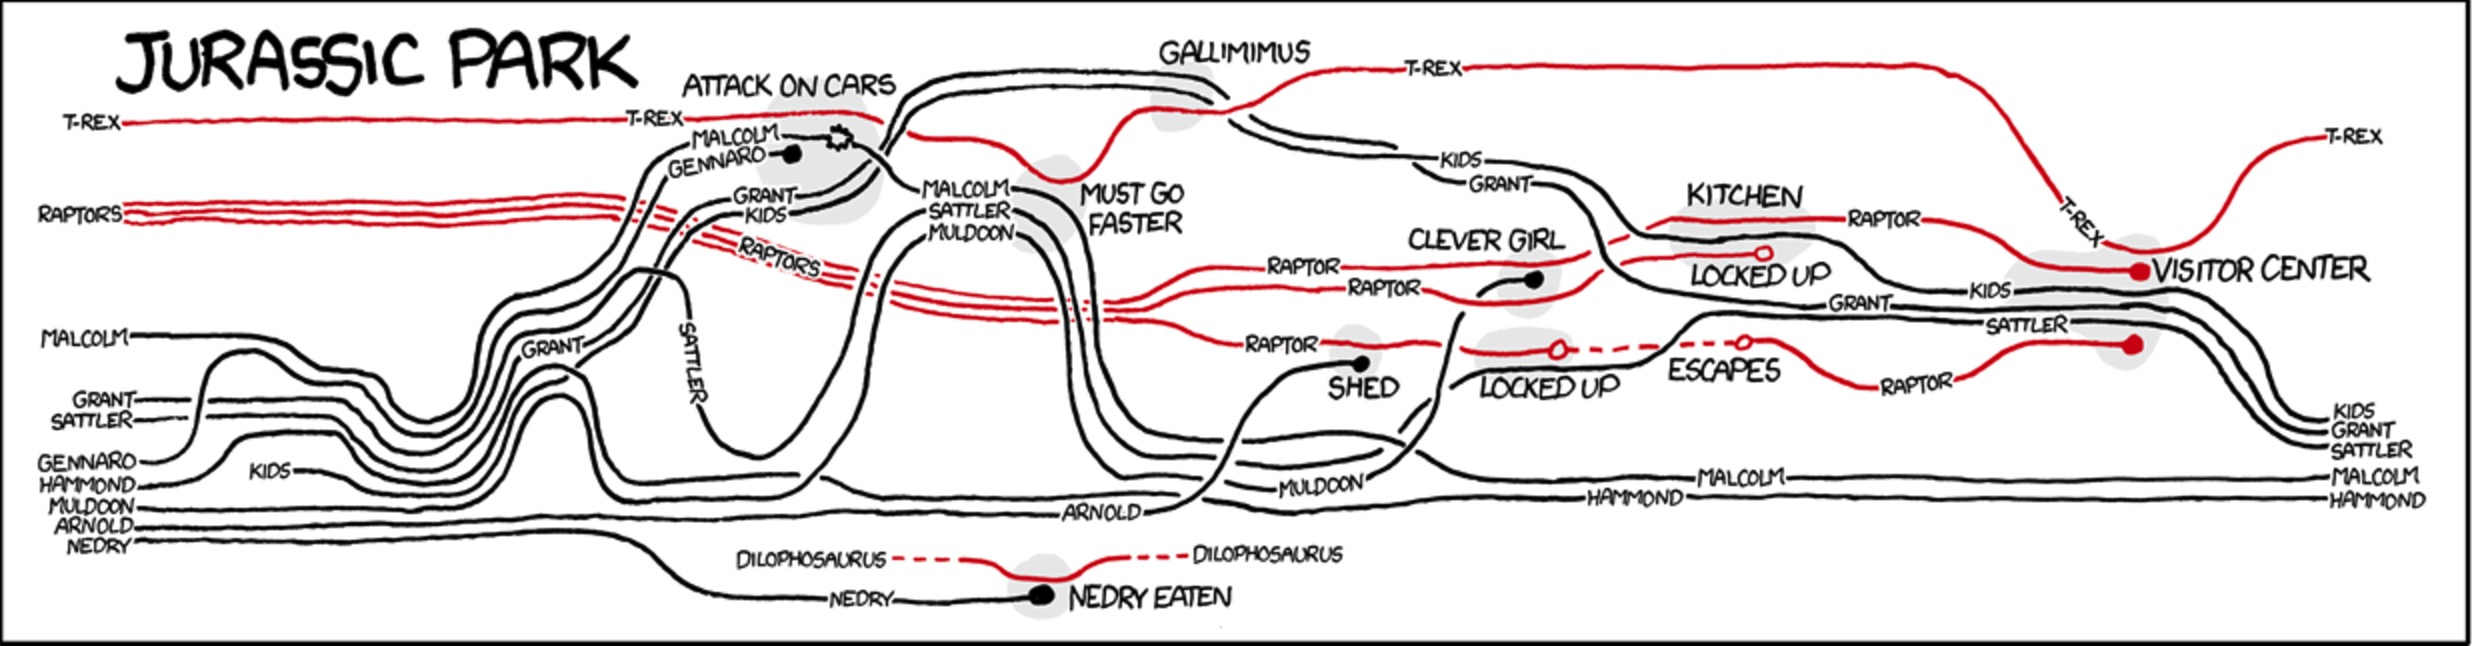
\includegraphics[width=15cm]{xkcd_jurassic_park}
	\caption{Jurassic park 人物关系手绘叙事图,X轴表示时间,垂直方向的分组表示在该时间点,人物之间有交互}
	\label{xkcd}
\end{figure}
% END == XKCD 手绘图

本章节我们将研究如何将这类手绘的叙事图(Narrative Chart)应用在新闻故事的人物关系可视化中,并研究如何实现由语料库自动生成Narrative Chart。要实现这一目标,我们需要将任务细分为以下几个子任务。首先,我们需要分析 Narrative Chart 由哪些核心的要素组成,以及这些要素之间的关系;其次,我们需要研究如何从语料库中自动抽取出 Narrative Chart 所需的要素,并规范化数据格式供图表生成系统使用;最后,我们需要研究通过何种技术将得到的 Narrative Chart 要素数据渲染成图表,并设计一系列算法,解决图表生成过程中遇到的各种问题。

\subsection{Narrative Chart 要素分析}

\subsubsection{角色 Character}
角色(Character 或是 Entity)是指故事中出现的人物,动物或其它角色。具体到新闻语料,角色是指新闻中出现的人、组织机构、国家等命名实体,它们一起构成了新闻故事六要素(时间、地点、人物、起因、经过和结果)之一的人物。电影、小说和新闻事件等通常都会有一个主角 (Main Character),所有的故事都围绕着主角展开和发展。因此,在我们的 Narrative Chart 也需要将主角(Main Character)与普通角色(Normal Character)区分开来。

\subsubsection{角色线索 Character Thread}
角色线索(Character Thread)是指串连角色从第一次出现到最后一次出现的一条时间轴上的连线。每一条角色线索都可以看作是故事在一个维度的体现,它反应了故事在该维度上的发展和变化。两条或多条角色线索可能在一个或多个时间点交叉,表示这这两个或多个角色在当前时间点共同出现在故事中,在该时间点产生了关联。

\subsubsection{场景 Scene}
场景(Scene)是指一个或多个角色在某个时间点发生的事情,每一个场景都是故事发展的一个新的阶段,表示故事的最新动态。如果某个场景中出现了两个或多个角色,那么该时间点在 Narrative Chart 中体现为两个角色线索的交叉点。

\subsection{Narrative Chart 要素抽取}
本小节,我们介绍如何从语料库中自动抽取角色(即:命名实体)信息,并定义表示 Narrative Chart 要素的数据格式。

\subsubsection{命名实体抽取 Named Entity Extraction}
实验中,我们只保留出现次数大于10次的角色。

\subsubsection{场景构建 Scene Construction}
场景构建的目的是为从语料库中抽取的命名实体建立关联关系,从而可以将其在 Narrative Chart 中予以表示。

实验中,我们设置时间跨度为一周,在这一周内如果两个角色有同时出现在一篇报道中,则创建一个场景,如果在这一周内两个角色同时出现在多个场景中,在 Narrative Chart 中为了保证图表的可读性,我们也仅展示一个场景,但是点击该场景,可以显示所有详细的报道情况。

\subsection{Narrative Chart 图表生成}

 \subsubsection{角色聚类 Characer Clustering}
为了凸显主要角色对于故事的重要性,我们需要用特俗的方式来呈现主要角色,以区别于普通角色。一种有效的方式是,将表示主要角色的Thread线条加粗并且用更加明显的颜色(如:红色)来标记。DBSCAN (Density Based Spatial Clustering of Applications with Noise)
 
 \subsubsection{角色线索排序 Character Thread Ordering}
 为了让 Narrative Charts 更好的呈现角色线索之间的关系,我们需要对 Character Thread 进行排序,使得这些 Thread 之间的非场景交叉尽可能减少,显然这个问题随着 Thread 数量的增加求解最佳解是一个 NP-Hard 问题。因此我们提出了一个启发式的试错算法,让最红的解向最优解不断靠近。



\section{主题变迁可视化}